% Final Spanish edition. 11pt, one column, 1-inch margins.
\documentclass[11pt]{article}
\usepackage[utf8]{inputenc}
\usepackage[T1]{fontenc}
\usepackage[spanish,es-nodecimaldot,es-noshorthands]{babel}
\usepackage[margin=1in]{geometry}
\usepackage{amsmath,amssymb,amsthm,booktabs,array,longtable,graphicx}
\usepackage[round]{natbib}
\usepackage[colorlinks=true,allcolors=blue!50!black]{hyperref}
\usepackage{xcolor}
\newtheorem{proposition}{Proposición}
\theoremstyle{definition}\newtheorem{assumption}{Supuesto}
\newcolumntype{L}[1]{>{\raggedright\arraybackslash}p{#1}}
\newcommand{\R}{\mathbb R}
\newcommand{\E}{\mathbb E}
\newcommand{\threshold}{0.640}
\newcommand{\betaZero}{0.130}
\newcommand{\betaOne}{-0.085}
\newcommand{\riskMin}{8.89}
\newcommand{\riskMax}{23.80}
\newcommand{\effortMin}{0.224}
\newcommand{\effortMax}{0.400}
\newcommand{\cohortSlope}{0.130}
\newcommand{\stockSlope}{-0.034}

\title{El precio relativo del crédito como señal de morosidad:\\
\large evaluación crediticia, restricciones y composición de cartera}
\author{Fabián Matías Galarza Chumbe\thanks{Universidad del Pacífico.
Proyecto final de AI and Economic Modeling, Línea B. El artículo desarrolla
el fundamento teórico de la investigación sobre precio relativo y morosidad
iniciada con William Brandon Grados Taco. Materiales de reproducción:
\url{https://github.com/fgalarzac/ai-project}. El apéndice documenta la
colaboración con inteligencia artificial.}}
\date{24 de noviembre de 2026}
\begin{document}
\maketitle
\begin{abstract}
El precio de los créditos nuevos se observa antes que su desempeño y puede
aportar información para la supervisión bancaria. Su relación con la morosidad
futura, sin embargo, depende de mecanismos que actúan en sentidos opuestos.
Este artículo resuelve la elección de evaluación crediticia de un banco,
condicionada en su precio relativo frente a otros bancos. Con selección
adversa lineal y costo cuadrático, la pendiente del riesgo es $a-g^2/c$
únicamente cuando la solución es interior: $a$ representa la selección de
solicitantes y $g^2/c$ la respuesta de evaluación. La capacidad limitada y
el piso de probabilidad modifican esa pendiente. Un cambio de signo por
opacidad requiere condiciones explícitas de cruce e interioridad. Al agregar
créditos nuevos y antiguos, la composición de cartera puede invertir el signo
del riesgo de originación. Tres proposiciones, sus demostraciones completas
y comprobaciones simbólicas y numéricas establecen estas condiciones. Los
resultados ofrecen una interpretación del indicador para la banca peruana;
las simulaciones son ilustrativas y no constituyen una estimación predictiva.
\end{abstract}

\section{Introducción}
El precio de un préstamo se conoce al originarlo; su desempeño crediticio se
revela más tarde. Esta diferencia temporal hace relevante preguntar si una
tasa inusualmente alta frente a la de bancos comparables permite anticipar
morosidad. Para un supervisor, una señal de ese tipo puede orientar el examen
de una entidad antes de que el deterioro sea visible en su balance. La
pregunta es especialmente pertinente cuando los datos disponibles combinan
tasas de colocaciones recientes con indicadores de calidad de una cartera
que contiene créditos de distintas edades.

El signo de la relación no es inmediato. Una tasa mayor puede atraer
solicitantes más riesgosos, pero también aumenta el beneficio de evitar un
crédito en atraso y, con ello, el incentivo del banco a evaluar. Además, una
reducción de nuevas colocaciones cambia su peso en el saldo total. Si esas
colocaciones son más riesgosas que la cartera antigua, su menor participación
puede reducir la morosidad agregada aun cuando empeore su riesgo individual.
Selección, evaluación y composición son, por tanto, mecanismos distintos que
deben separarse al interpretar el precio relativo.

El artículo desarrolla el modelo económico de esta interpretación para la
pregunta de la banca múltiple peruana. El banco elige cuánto evaluar un
crédito, dado su precio y la tecnología del segmento. La selección adversa
eleva el riesgo previo con el precio; la evaluación lo reduce, a un costo
creciente. Dos restricciones delimitan el esfuerzo: la capacidad operativa y
la imposibilidad de obtener una probabilidad negativa. Resolver el problema
con ambas restricciones permite identificar cuándo responde el esfuerzo y
cuándo cambia únicamente la calidad de los solicitantes.

El primer resultado caracteriza un máximo único y distingue tres regímenes.
En el interior, la selección domina si $a>g^2/c$, donde $a$ mide la sensibilidad
del riesgo previo al precio, $g$ la productividad de evaluar y $c$ la escala
del costo cuadrático. Cuando se agota la capacidad, el esfuerzo deja de
responder y la pendiente del riesgo es $a$. Cuando se alcanza el piso de
probabilidad, esa pendiente es cero. El segundo resultado establece un
umbral único por opacidad bajo condiciones de continuidad, descenso estricto,
cruce e interioridad. El tercero deriva la transmisión al ratio de cartera y
una condición exacta para que la composición invierta el signo.

El antecedente empírico más próximo es \citet{morgan2003}, que encuentra
información sobre desempeño posterior en las tasas de nuevos préstamos
comerciales e industriales. La contribución del presente artículo es precisar
las condiciones necesarias para interpretar una señal de ese tipo cuando la
evaluación es endógena y la variable observada es un ratio de saldo. La
solución global y la identidad de composición articulan ingredientes conocidos
en un problema bancario explícito. El análisis es teórico y condicionado en
precio; su aplicación predictiva al Perú requiere una contrastación empírica
separada.

La exposición sigue el orden del mecanismo. La Proposición~\ref{p:global}
resuelve la decisión de esfuerzo. La Proposición~\ref{p:threshold} compara
segmentos con distinta opacidad al mismo precio. La Proposición~\ref{p:stock}
agrega el riesgo resultante a una cartera antigua. Las simulaciones permiten
examinar las condiciones y los casos de fracaso de cada resultado; la
discusión final extrae sus implicaciones para medición y pronóstico.

\section{Evidencia institucional y medición}
\subsection{Tasas de colocación e indicadores de cartera}
La Superintendencia de Banca, Seguros y AFP (SBS), autoridad de supervisión
financiera peruana, publica tasas efectivas anuales por empresa y operación. La sección 3
de su metodología define promedios de operaciones de los últimos treinta días
útiles, ponderados por los montos desembolsados \citep{sbsmetodo}. Son tasas
sobre \emph{flujos}: describen créditos recientes y difieren de las tasas
sobre saldos vigentes. Como las ventanas de treinta días útiles pueden
superponerse entre cierres mensuales, tampoco equivalen a una cohorte exacta
del mes calendario. Agrupar por tipo de operación, plazo y moneda mejora la
comparabilidad, aunque persisten diferencias de garantías, deudores y relaciones
comerciales.

La evidencia peruana ilustra por qué estas distinciones importan.
\citet{choy2015} documenta, para 2010--2014, el papel de costos operativos y
riesgo en las diferencias de tasas entre segmentos. Una tasa elevada puede
reflejar esos componentes además de selección adversa. Asimismo, cartera
atrasada, atraso mayor de noventa días y cartera de alto riesgo (CAR) miden
eventos distintos. Vincular una tasa con una probabilidad requiere precisar
el evento, la población y el horizonte de observación.

El Reporte de Estabilidad Financiera de noviembre de 2024 del Banco Central
de Reserva del Perú (BCRP) presenta
indicadores de saldo y seguimiento por cosechas, en su cuadro 2.2 y gráfico
2.7 \citep{bcrp2024}. La Figura~\ref{fig:context} reproduce cuatro series del
cuadro y muestra diferencias persistentes entre segmentos. La CAR ajustada
incluye castigos de los últimos doce meses y corresponde al sistema financiero,
un universo más amplio que la banca múltiple. Se utiliza como contexto
institucional, con su definición original; no como calibración del modelo ni
como sustituto de la variable objetivo de la tesis.

\begin{figure}[htbp]
\centering
\begin{minipage}{.96\linewidth}
\centering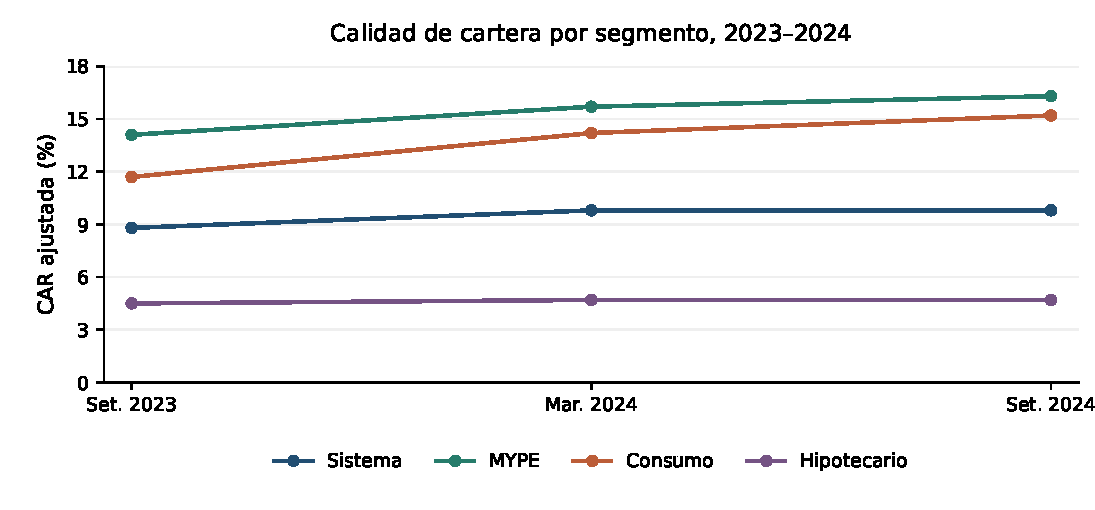
\includegraphics[width=\linewidth]{../code/figures/public_context.pdf}
\caption{Calidad de cartera por segmento. CAR ajustada por castigos de los
últimos doce meses, en porcentaje; sistema financiero. MYPE designa los
créditos a micro y pequeñas empresas.
Fuente: BCRP, Reporte de Estabilidad Financiera, noviembre de 2024,
cuadro 2.2, p. 21. La transcripción reproducible se encuentra en
\texttt{code/data/}.}\label{fig:context}
\end{minipage}
\end{figure}

El análisis cuantitativo del artículo consiste en simulaciones del modelo y
en esta transcripción acotada de estadísticas públicas. Los parámetros de las
simulaciones son hipotéticos. La interpretación económica de sus resultados
se distingue de una estimación de parámetros o de una evaluación de pronósticos.

\subsection{Definición del precio relativo}
Sea $j$ un banco, $s$ una celda de tipo de crédito, modalidad o tramo de plazo
y moneda, y $t$ la fecha del reporte. Denote por $i_{jst}$ su tasa anual en
decimales y por $b_{st}$ una base común en la misma moneda. Sea
$\mathcal P_{-j,st}$ el conjunto de otros bancos con observación válida y
$n_{-j,st}$ su tamaño. El precio relativo se define como
\begin{equation}\label{eq:D}
D_{jst}=(i_{jst}-b_{st})-
\frac{1}{n_{-j,st}}\sum_{k\in\mathcal P_{-j,st}}(i_{kst}-b_{st})
=i_{jst}-\frac{1}{n_{-j,st}}\sum_k i_{kst}.
\end{equation}
El banco evaluado queda fuera de su referencia. Un valor $D=0.02$ indica una
tasa dos puntos porcentuales superior al promedio de pares. El promedio
simple permite construir una comparación transparente cuando no se observan
desembolsos por tramo; difiere de una tasa del sistema ponderada por
operaciones. Una aplicación empírica debe fijar las reglas de comparabilidad
y exigir al menos tres pares válidos antes de evaluar su desempeño predictivo.

La mediana constituye una medida de sensibilidad. Reduce la influencia de
tasas extremas, pero cambia el comparador y puede modificar incluso el signo
de la brecha. Con tasas de pares hipotéticas de 8, 9, 10 y 25\%, una tasa
propia de 12\% está un punto por debajo del promedio y 2.5 puntos por encima
de la mediana. Ambas diferencias se verifican en el código. La elección del
comparador debe preceder a la evaluación del error de pronóstico.

La cancelación de la base común en \eqref{eq:D} es algebraica. No elimina las
exposiciones heterogéneas a un mismo shock. Si $i_j=b+\lambda_j z+v_j$, donde
$z$ es el shock agregado, $\lambda_j$ la exposición del banco y $v_j$ su
componente específico, la diferencia frente a pares conserva
$(\lambda_j-\bar\lambda_{-j})z+(v_j-\bar v_{-j})$. Las barras representan
promedios de los otros bancos. Por ello, fondeo, costos, clientela y márgenes
pueden seguir afectando la brecha. Un cambio en el conjunto de pares también
puede mover $D$ sin que cambie la tasa propia. La comparación relativa mejora
la descripción del precio, pero no constituye una estrategia de identificación
causal.

\section{Literatura relacionada y mecanismos}
\citet{morgan2003} encuentra contenido predictivo de las tasas de nuevos
préstamos comerciales e industriales de Estados Unidos para su desempeño
posterior y sus calificaciones supervisoras. El hallazgo, publicado en 2003,
motiva el uso informativo del precio. El presente análisis estudia una
distinción adicional: la calidad de una cohorte nueva y el ratio de saldo de
una cartera pueden responder de manera diferente. La evidencia estadounidense
no establece por sí sola el signo de esa relación para bancos peruanos.

El mecanismo de selección se relaciona con \citet{stiglitz1981}, p. 393:
el precio altera la composición y los incentivos de quienes solicitan crédito.
El modelo resume el primer canal mediante una sensibilidad positiva del riesgo
previo al precio. \citet{broecker1990} estudia pruebas imperfectas y competencia
entre bancos; \citet{ruckes2004} relaciona estándares crediticios y competencia
con las perspectivas económicas; y \citet{dellariccia2006} distingue regímenes
de evaluación y agrupación de prestatarios. Estos artículos publicados aportan
el contexto teórico. La contribución se concentra en una decisión de evaluación
condicionada en precio y en su vínculo con la composición de cartera.

Para la medición peruana, \citet{yamunaque2024} construye una medida del
deterioro de créditos inicialmente normales durante doce meses y la distingue
del ratio contable de morosidad. La referencia se cita como Documento de
Trabajo 2024-015 del BCRP, estado editorial verificado en su catálogo. Esta
distinción respalda la elección explícita de evento y horizonte en el modelo:
una probabilidad de deterioro no puede equipararse automáticamente a cualquier
serie publicada de morosidad. \citet{clark2007}, por su parte, desarrolla una
comparación de pronósticos de modelos anidados que resulta pertinente para
evaluar posteriormente la información incremental del precio relativo.

Los mecanismos generan patrones observables diferentes. Cuando domina la
selección, precios mayores se asocian con peor calidad de nuevas cosechas,
manteniendo constante la evaluación. Cuando domina la evaluación, el mayor
precio debe acompañarse de una respuesta efectiva del esfuerzo y de menor
riesgo posterior, siempre que la capacidad permita esa respuesta. Cuando
domina la composición, el cambio de signo aparece al agregar cohortes y
depende de sus pesos. Distinguir esos patrones requiere información sobre
cosechas, saldos, evaluación y garantías; las tasas promedio, por sí solas,
no identifican cuál de ellos opera.

\section{Modelo}\label{sec:model}
\subsection{Agentes, información, unidades y cronología}
El único agente que optimiza en este modelo es un banco neutral al riesgo.
Los solicitantes y los bancos pares determinan una calidad y una referencia
reducidas; no se modela su juego estratégico. El supervisor observa $D$ y más
tarde un ratio de cartera, pero no el esfuerzo ni toda la composición de riesgo.
La opacidad $\kappa\in[0,1]$ es una característica exógena del segmento: un
valor mayor representa menor información verificable inicial. El índice organiza la comparación teórica entre segmentos y no se identifica
automáticamente con una categoría observada, como microempresa.

La cronología es: primero se fijan segmento, tecnología y precio observado;
después se forma el conjunto de solicitantes y el banco observa su riesgo
medio; luego elige esfuerzo antes de originar; finalmente se realiza el
estado crediticio y se observa la cartera al horizonte $h$. El banco conoce
los parámetros al decidir. La incertidumbre de desempeño permanece y se
integra en su objetivo. El precio es un argumento del problema de continuación,
no una variable resuelta en equilibrio.

$q^0$ y $q$ son probabilidades sin unidades, referidas al mismo evento y
horizonte para una cohorte estandarizada. $e$ y $\kappa$ son índices. $D$ se
mide en unidades de tasa anual decimal. Los pagos y costos se normalizan por
sol de crédito. La sensibilidad monetaria del premio de desempeño a una unidad
de $D$ se normaliza a uno. Esto es una simplificación de remuneración, no una
conversión exacta de tasas efectivas a cualquier plazo contractual.

La interpretación de las pruebas exige distinguir tres operaciones. Al elegir
$e$, el banco mantiene fijos $D$ y $\kappa$: compara esfuerzos para un mismo
precio y segmento. Al calcular $\partial_Dq^*$, compara problemas con precios
cercanos, dejando fijo el segmento y permitiendo que cambie el esfuerzo
óptimo. Solo en la Proposición~\ref{p:threshold} se comparan distintos valores
de $\kappa$, siempre al mismo precio $D_0$. La prima de $M'$ se refiere a $D$;
las primas de $g'$ y $c'$ en el análisis de opacidad se refieren a $\kappa$.

La tabla siguiente reúne la notación y sus unidades. Los objetos de cartera
intervienen a partir de la Proposición~\ref{p:stock}; no intervienen en la elección inicial
del esfuerzo.
\begin{center}\small
\begin{tabular}{@{}L{.15\linewidth}L{.51\linewidth}L{.27\linewidth}@{}}
\toprule Símbolo & Significado & Unidad o restricción\\\midrule
$D$ & Tasa propia menos promedio simple de pares & Tasa anual decimal\\
$\kappa$ & Opacidad exógena del segmento & Índice en $[0,1]$\\
$\bar q,a$ & Riesgo de referencia y sensibilidad de selección & Probabilidad; $a>0$\\
$q^0,q,q^*$ & Riesgo previo, posterior y posterior óptimo & Mismo evento y horizonte\\
$e,\bar e,u$ & Esfuerzo, capacidad y máximo esfuerzo factible & Índices no negativos\\
$g,c$ & Productividad y escala del costo de evaluación & Ambos positivos\\
$R,\bar R,F$ & Premio por desempeño, premio de referencia y costo fijo & Pagos por sol de crédito\\
$z$ & Esfuerzo deseado sin restricciones: $gR/c$ & Índice de esfuerzo\\
$H,\beta$ & Fuerza de evaluación $g^2/c$ y pendiente neta $a-H$ & Riesgo por unidad de $D$\\
$\beta_D$ & Derivada de $q^*$ en el régimen efectivo & Riesgo por unidad de $D$\\
$B_0,B,B_1$ & Saldos antiguo, nuevo y nuevo cuando $D=0$ & Misma unidad monetaria\\
$m_0,w,M$ & Atraso antiguo, peso nuevo y ratio total & Fracciones en $[0,1]$\\
$\varepsilon$ & Sensibilidad proporcional de $B$ al precio & Por unidad de $D$\\
\bottomrule
\end{tabular}
\end{center}

\begin{assumption}[Selección y dominio]\label{as:selection}
Para cada $\kappa$ fijo, $a=a(\kappa)>0$, $\bar q\in(0,1)$ y $D$ pertenece
a un intervalo compacto $\mathcal D$. La probabilidad previa es
$q^0(D,\kappa)=\bar q+a(\kappa)D\in[0,1]$ en todo $\mathcal D$.
\end{assumption}
La forma afín es una aproximación local al cambio de solicitantes. Una subida
de un punto porcentual es $\Delta D=0.01$: cambia la probabilidad en $0.01a$
unidades, equivalentes a $a$ puntos porcentuales. Por ejemplo, con $a=0.18$
el cambio es $0.0018$ de probabilidad, es decir, $0.18$ puntos porcentuales.
No se extrapola fuera del dominio admisible. La pendiente positiva representa
selección adversa, no una ley empírica universal ni una respuesta derivada de
un problema explícito de cada deudor.

La restricción de probabilidad también fija qué precios se pueden comparar.
Restar $\bar q$ y dividir por $a>0$ da
\[
0\le\bar q+aD\le1
\quad\Longleftrightarrow\quad
-\frac{\bar q}{a}\le D\le\frac{1-\bar q}{a}.
\]
El dominio compacto $\mathcal D$ se elige dentro de ese intervalo y debe
respetar además el pago positivo del Supuesto~\ref{as:payoff}. No se pretende
describir cualquier tasa posible con una probabilidad afín.

\begin{assumption}[Tecnología, capacidad y costo]\label{as:technology}
$g=g(\kappa)>0$, $c=c(\kappa)>0$ y $\bar e\ge0$ son finitos. Para un volumen
normalizado de créditos, $q(D,e,\kappa)=q^0(D,\kappa)-g(\kappa)e$ y el costo
es $c(\kappa)e^2/2$. La elección factible cumple
\[
0\le e\le u(D,\kappa):=\min\{\bar e,q^0(D,\kappa)/g(\kappa)\}.
\]
\end{assumption}
El límite $q^0/g$ evita probabilidades negativas. La capacidad $\bar e$ puede
representar personal o tiempo de verificación. Evaluar incluye comprobación
y condiciones contractuales que reducen el riesgo de los créditos colocados.
El modelo mantiene el volumen fijo respecto del esfuerzo: no estudia la
composición endógena de rechazos ni su costo de reemplazo. Si evaluar elimina
solicitantes sin reemplazo, el volumen dependería de $e$ y la solución cambiaría.
La tecnología lineal puede llegar a riesgo cero, una frontera matemática cuyo
realismo es limitado; no se presenta como objetivo factible de un supervisor.

La segunda cota se obtiene directamente de $q\ge0$: como $g>0$,
$q^0-ge\ge0$ equivale a $e\le q^0/g$. La primera cota, $e\le\bar e$,
es tecnológica. Cumplir ambas significa tomar su mínimo. Además, $e\ge0$
asegura $q\le q^0\le1$. El conjunto $0\le e\le u$ impide tanto esfuerzo
negativo como riesgo negativo, y respeta simultáneamente la capacidad.

\begin{assumption}[Remuneración y problema condicionado]\label{as:payoff}
El premio normalizado por desempeño es $R(D)=\bar R+D>0$ y $F$ es un costo
por unidad independiente de $e$. El banco resuelve
\begin{equation}\label{eq:problem}
\max_{e\in[0,u(D,\kappa)]}\pi(e;D,\kappa)
=[1-q^0(D,\kappa)+g(\kappa)e]R(D)-F-\frac{c(\kappa)}2e^2.
\end{equation}
El precio, la referencia de pares y $\kappa$ se mantienen fijos al evaluar
desviaciones de esfuerzo.
\end{assumption}
El costo $F$ no afecta el óptimo de esfuerzo. Un volumen estrictamente
positivo que multiplique todo el objetivo tampoco lo afecta si no depende
de $e$. La participación o decisión de no prestar no está resuelta: el
resultado se refiere a una unidad que el banco ya contempla originar.
La remuneración supone que evitar el evento adverso mejora el pago esperado.
Recuperaciones, seguros y garantías que varían con precio o esfuerzo exigirían
modificar este premio. El horizonte del evento y el flujo contractual deben
ser compatibles en una implementación empírica.

Para leer el objetivo, empiece por $1-q^0+ge=1-q$: es la probabilidad de
evitar el evento adverso. Multiplicarla por $R$ da el premio esperado. Después
se restan el costo fijo $F$ y el costo de evaluar. Una unidad adicional de
esfuerzo aporta $gR$ de beneficio marginal y cuesta $ce$. Al subir el precio,
$R$ aumenta; al subir el esfuerzo, su costo marginal aumenta. Ese contraste
explica la respuesta del banco, pero todavía no dice si el esfuerzo deseado
cabe dentro de las restricciones.

\section{Resultados y demostraciones completas}
\subsection{Evaluación óptima con todas sus restricciones}
\begin{proposition}[Solución global y pendientes por régimen]\label{p:global}
Bajo los Supuestos~\ref{as:selection}--\ref{as:payoff}, existe un único máximo
en \eqref{eq:problem}. Es
\begin{equation}\label{eq:opt}
e^*=\min\left\{\frac{gR(D)}c,\bar e,\frac{q^0(D)}g\right\},\qquad
q^*=\max\left\{0,q^0(D)-g\min\left\{\bar e,\frac{gR(D)}c\right\}\right\}.
\end{equation}
Para $\kappa$ fijo, en cualquier intervalo abierto con desigualdades estrictas
que mantengan el régimen, las pendientes son
\begin{equation}\label{eq:regimes}
\frac{\partial q^*}{\partial D}=
\begin{cases}
a-g^2/c,&gR/c<\bar e\ \text{y}\ gR/c<q^0/g,\\
a,&\bar e<gR/c\ \text{y}\ \bar e<q^0/g,\\
0,&q^0/g<gR/c\ \text{y}\ q^0/g<\bar e.
\end{cases}
\end{equation}
Si $\bar e=0$, $e^*=0$ y $q^*=q^0$, con pendiente $a$ en el interior del
dominio de $D$. En empates de restricciones la solución es continua y se usan
derivadas laterales; una derivada ordinaria puede no existir.
\end{proposition}
\begin{proof}
\textbf{Paso 1: hay una elección factible y el máximo es único.}\par
Fijamos $D$ y $\kappa$, de modo que $q^0,R,g,c,\bar e$ son constantes al
comparar esfuerzos. Como $q^0\ge0$, $g>0$ y $\bar e\ge0$, se cumple $u\ge0$.
El intervalo $[0,u]$ es no vacío y compacto y $\pi$ es continua: por el teorema
del valor extremo alcanza un máximo. Si $u=0$, solo se puede elegir $e=0$.
Si $u>0$, la segunda derivada es $\pi_{ee}=-c<0$; la concavidad estricta en
un intervalo convexo impide dos máximos distintos.

\textbf{Paso 2: el primer orden identifica el esfuerzo deseado.}\par
Derivar respecto de $e$, manteniendo fijos precio y segmento, da
\[
\pi_e=gR-ce,\qquad \pi_e=0\ \Longleftrightarrow\ e=z:=gR/c>0.
\]
La igualdad entre beneficio y costo marginal no demuestra que $z\le u$.
Por eso $z$ es todavía un candidato sin restricciones.

\textbf{Paso 3: resolver el problema restringido.}\par
Completar el cuadrado muestra qué hacer cuando el candidato no es factible:
\begin{align*}
gRe-\frac c2e^2
 &=-\frac c2\left[e^2-2\frac{gR}{c}e\right]
  =-\frac c2\left[(e-z)^2-z^2\right],\\
\pi(e)&=\underbrace{(1-q^0)R-F+\frac{(gR)^2}{2c}}_{\text{constante respecto de }e}
              -\frac c2(e-z)^2.
\end{align*}
Puesto que $c>0$, maximizar $\pi$ equivale a minimizar $(e-z)^2$ en $[0,u]$.
Si $z\le u$, el único punto a distancia cero es $e=z$. Si $z>u$, para todo
$e<u$ se tiene $z-e>z-u>0$ y, al elevar al cuadrado,
$(e-z)^2>(u-z)^2$. El único máximo es entonces $e=u$. Esto incluye el caso
$u=0$; si $z=u$, ambos argumentos identifican el mismo punto. En consecuencia,
\[
e^*=\min\{z,u\}=\min\{gR/c,\bar e,q^0/g\}.
\]

\textbf{Paso 4: sustituir en la probabilidad y comprobar sus cotas.}\par
Definimos $v=\min\{\bar e,gR/c\}\ge0$. Si $v\le q^0/g$, entonces $e^*=v$ y
$q^*=q^0-gv\ge0$. Si $v>q^0/g$, entonces $e^*=q^0/g$ y $q^*=0$. Los dos
casos son exactamente $q^*=\max\{0,q^0-gv\}$. Además, como $e^*\ge0$ y
$g>0$, $q^*\le q^0\le1$. Así se obtiene la segunda fórmula y se comprueba
que se trata de una probabilidad válida.

\textbf{Paso 5: derivar dentro de cada régimen.}\par
Con $\kappa$ fijo, las desigualdades estrictas se conservan en un entorno
del precio considerado. Se puede derivar la expresión que allí está activa:
\begin{align*}
\text{Interior: }q^*&=\bar q+aD-\frac{g^2}{c}(\bar R+D),
 &\partial_Dq^*&=a-g^2/c;\\
\text{Capacidad: }q^*&=\bar q+aD-g\bar e,
 &\partial_Dq^*&=a;\\
\text{Piso: }q^*&=0,
 &\partial_Dq^*&=0.
\end{align*}
En el interior, $\partial_De^*=g/c$: al multiplicar por la productividad $g$
se obtiene la reducción marginal $g^2/c$. Con capacidad agotada el esfuerzo
ya no responde. En el piso, el riesgo no puede seguir bajando.

\textbf{Paso 6: capacidad cero y empates.}\par
Si $\bar e=0$, el conjunto factible es $\{0\}$, por lo que $e^*=0$ y
$q^*=q^0$; en el interior del dominio su derivada es $a$. Para capacidad
general, las funciones afines que entran al mínimo son continuas. El mínimo
y el máximo de un número finito de funciones continuas son continuos: no
hay saltos en $e^*$ ni en $q^*$. También son funciones afines por tramos.
En cada lado de un empate se activa una de esas expresiones, de modo que
existen las pendientes laterales. Si dos expresiones coinciden en todo un
intervalo, tienen la misma pendiente y no generan un problema nuevo. Cuando
las pendientes de ambos lados difieren, la derivada ordinaria no existe;
el ejemplo de capacidad de la sección~\ref{sec:sim} muestra ese caso.
\end{proof}

La intuición de $g^2/c$ tiene dos pasos: un mayor precio eleva el esfuerzo en
$g/c$ en el interior y cada unidad de esfuerzo reduce riesgo en $g$. Cuando
la capacidad está agotada, la primera respuesta desaparece. En consecuencia,
un banco con alta productividad puede mostrar pendiente positiva si enfrenta
capacidad escasa. La condición $g^2/c>a$ por sí sola no basta globalmente.

\paragraph{Un recorrido numérico de la decisión.}
El cálculo puede seguirse con los parámetros hipotéticos de la simulación:
$\bar q=0.28$, $a=0.18$, $g=\sqrt{0.05}$, $c=1$, $\bar R=1.10$ y
$\bar e=0.50$. En $D=0$, $q^0=0.28$ y $R=1.10$. El candidato es
$gR/c\simeq0.246$, menor que la capacidad $0.50$ y que la cota
$q^0/g\simeq1.252$: el banco es interior. Evaluar reduce el riesgo en
$ge^*=0.055$, por lo que queda $q^*=0.225$. Localmente, un punto porcentual
más de precio añade $0.18$ puntos porcentuales por selección y resta $0.05$
por evaluación; el resultado neto es $0.13$ puntos porcentuales. El cálculo
solo ilustra las unidades y el mecanismo, sin calibración con datos peruanos.

\subsection{Qué requiere un umbral por opacidad}
Defina $H(\kappa)=g(\kappa)^2/c(\kappa)$ y
$\beta(\kappa)=a(\kappa)-H(\kappa)$.
\begin{assumption}[Condiciones suficientes para el cruce]\label{as:cross}
En $\kappa\in[0,1]$, $a,g,c$ son continuas y positivas. La función
$a-H$ es estrictamente decreciente y satisface $a(0)>H(0)$ y $a(1)<H(1)$.
Al precio $D_0$ que se compara se cumplen estrictamente las dos condiciones
de interioridad de la primera línea de \eqref{eq:regimes} para todo $\kappa$.
\end{assumption}
\begin{proposition}[Umbral condicional]\label{p:threshold}
Bajo los Supuestos~\ref{as:selection}--\ref{as:cross}, existe un único
$\kappa^*\in(0,1)$ con $\partial_Dq^*(D_0,\kappa^*)=0$. La derivada es
positiva para $\kappa<\kappa^*$ y negativa para $\kappa>\kappa^*$.
\end{proposition}
\begin{proof}
\textbf{Paso 1: continuidad de la pendiente neta.}\par
Por S4, $a,g,c$ son continuas en $[0,1]$ y $c$ es estrictamente positiva.
El cuadrado y el cociente conservan continuidad cuando el denominador no se
anula. Por tanto $H=g^2/c$ y $\beta=a-H$ son continuas.

\textbf{Paso 2: existencia de un cero interior.}\par
S4 implica $\beta(0)=a(0)-H(0)>0$ y $\beta(1)=a(1)-H(1)<0$. El teorema
del valor intermedio da un $\kappa^*\in(0,1)$ tal que $\beta(\kappa^*)=0$.
Es interior porque ninguno de los dos extremos tiene valor cero.

\textbf{Paso 3: unicidad y orden de los signos.}\par
Si $x<y$ fueran dos ceros, el descenso estricto daría
$0=\beta(x)>\beta(y)=0$, una contradicción. Para cualquier
$\kappa<\kappa^*$, la misma propiedad da
$\beta(\kappa)>\beta(\kappa^*)=0$; para $\kappa>\kappa^*$ da la desigualdad
inversa. Así se obtienen un único cero y los signos a cada lado.

\textbf{Paso 4: volver a la derivada del riesgo.}\par
El cero anterior es el de una función de primitivas. Para identificarlo
con el objeto económico, falta usar la última parte de S4: al precio común
$D_0$ el esfuerzo es interior para toda $\kappa$. La primera línea de
\eqref{eq:regimes} da entonces
$\partial_Dq^*(D_0,\kappa)=a(\kappa)-g(\kappa)^2/c(\kappa)=\beta(\kappa)$.
El cero único y sus signos son exactamente los del enunciado. Sin
interioridad, el cero de $\beta$ no bastaría para caracterizar la pendiente
del régimen efectivo.
\end{proof}

El Supuesto~\ref{as:cross} es una restricción económica contrastable, no el
significado de opacidad. Si las funciones son diferenciables,
\begin{equation}\label{eq:logs}
\frac{H'}H=2\frac{g'}g-\frac{c'}c.
\end{equation}
Por ejemplo, información inicial escasa podría dejar más margen para
verificación adicional, pero no demuestra $g'>0$. Si el acceso a información
es más difícil, es plausible $g'\le0$ y $c'\ge0$, con $H'\le0$. Puede no
haber cruce, o puede haberlo si $a$ cae suficientemente rápido. Ni $H'>0$ es
necesario por sí solo ni la mera continuidad asegura unicidad. Un criterio
suficiente más fuerte es $a'<0$, $H'>0$ y cruce de extremos.
El resultado final solo exige que $a-H$ decrezca estrictamente. La sensibilidad
estudia explícitamente una tecnología que empeora con opacidad.

\subsection{El puente entre una cohorte y el saldo de cartera}
Fijemos un horizonte $h$. $B_0>0$ es el saldo de créditos antiguos todavía
vigente en esa fecha y $m_0\in[0,1]$ su proporción en el estado de atraso
elegido. $B(D)>0$ es el saldo de la cohorte nueva que permanece en cartera a
$h$, después de amortización normal. Denote $w(D)=B(D)/(B_0+B(D))$.

Un ejemplo explica el peso sin derivadas. Si el saldo antiguo es cuatro y
el nuevo uno, el peso nuevo es $1/(4+1)=0.20$: el ochenta por ciento del
ratio corresponde a la cartera antigua. Mejorar o empeorar los créditos
nuevos no cambia el mismo porcentaje del saldo total. La magnitud depende
también de cuánto pesa esa cohorte.

\begin{assumption}[Contabilidad y maduración]\label{as:stock}
Al horizonte, el saldo de cada cohorte es determinista o se trata como
exposición de una población continua. El riesgo $q^*(D)$ coincide con la
fracción esperada de su saldo en el evento crediticio elegido, condicional
a seguir en cartera. La amortización y el tamaño del crédito no seleccionan
riesgo adicional no recogido en $q^*$. $B_0,m_0$ son constantes al variar $D$;
$B(D)>0$ es diferenciable. No hay castigos, ventas de cartera ni
reclasificaciones que alteren esta identidad en el ejercicio.
\end{assumption}
La compatibilidad exigida por el supuesto es sustantiva. Una
probabilidad de impago de por vida no equivale a la probabilidad de figurar
con atraso mayor de noventa días en una fecha dada. Hay que definir horizonte,
maduración, persistencia del atraso y permanencia del saldo. Si esos procesos
cambian con $D$, deben incluirse en $q^*$ o en la contabilidad ampliada.

\begin{proposition}[Transmisión y composición]\label{p:stock}
Bajo los Supuestos~\ref{as:selection}--\ref{as:payoff} y~\ref{as:stock}, el
ratio esperado de cartera es $M(D)=(1-w)m_0+wq^*(D)$. En cualquier régimen
diferenciable, escribiendo $\beta_D=\partial_Dq^*(D)$,
\begin{equation}\label{eq:stock}
M'(D)=w\beta_D+w'(q^*-m_0).
\end{equation}
Si $B$ es constante, el signo es el de $\beta_D$. Si $\beta_D\ne0$ y
$|w'(q^*-m_0)|<w|\beta_D|$, el signo también se conserva.
Con $B(D)=B_1e^{-\varepsilon D}$, $B_1>0$, $\varepsilon\ge0$,
\begin{equation}\label{eq:composition}
M'=w\{\beta_D-\varepsilon(1-w)(q^*-m_0)\}.
\end{equation}
En particular, $\beta_D>0$ y $q^*>m_0$ generan $M'<0$ si y solo si
$\varepsilon(1-w)(q^*-m_0)>\beta_D$.
\end{proposition}
\begin{proof}
\textbf{Paso 1: construir el ratio con saldos comparables.}\par
Bajo S5, el saldo esperado en atraso es $B_0m_0+Bq^*$. Su denominador
$B_0+B$ es determinista y positivo. Por eso se puede dividir la suma esperada
por ese saldo; no se intercambian sin justificación una esperanza de ratios
y un ratio de esperanzas. Separar los dos sumandos da
\[
M=\frac{B_0}{B_0+B}m_0+\frac{B}{B_0+B}q^*
  =(1-w)m_0+wq^*,\qquad 0<w<1.
\]

\textbf{Paso 2: identificar calidad y composición.}\par
Como $B_0,m_0$ son constantes respecto de $D$, la regla del producto da
\begin{align*}
M'&=-w'm_0+w'q^*+w\,\partial_Dq^*\\
  &=w\beta_D+w'(q^*-m_0),
\end{align*}
que es \eqref{eq:stock}. El primer término cambia la calidad de los créditos
nuevos manteniendo su peso; el segundo cambia el peso de una cohorte cuya
calidad difiere de la antigua.

\textbf{Paso 3: comprobar las dos reglas de conservación del signo.}\par
Si $B$ es constante, también lo es $w$, de modo que $w'=0$ y
$M'=w\beta_D$. Como $w>0$, ambos tienen el mismo signo, incluido el caso cero.
Para la segunda regla denote $T=w'(q^*-m_0)$, el término de composición.
Si $\beta_D>0$ y $|T|<w|\beta_D|=w\beta_D$, entonces
$M'=w\beta_D+T\ge w\beta_D-|T|>0$. Si $\beta_D<0$, entonces
$w|\beta_D|=-w\beta_D$ y
$M'\le w\beta_D+|T|<0$. La condición estricta evita que composición
anule o invierta la pendiente no nula.

\textbf{Paso 4: derivar el peso de la cohorte.}\par
La regla del cociente, usando $B_0'=0$, produce
\[
w'=\frac{B'(B_0+B)-BB'}{(B_0+B)^2}
   =\frac{B'B_0}{(B_0+B)^2}.
\]
En el caso exponencial, $B'= -\varepsilon B$. Al sustituir y reconocer
$B/(B_0+B)=w$ y $B_0/(B_0+B)=1-w$, resulta
$w'=-\varepsilon w(1-w)$. Insertar esto en \eqref{eq:stock} da
\eqref{eq:composition}.

\textbf{Paso 5: despejar la condición exacta de inversión.}\par
Puesto que $w>0$, el signo de $M'$ coincide con el del corchete:
\[
M'<0\quad\Longleftrightarrow\quad
\beta_D-\varepsilon(1-w)(q^*-m_0)<0
\quad\Longleftrightarrow\quad
\varepsilon(1-w)(q^*-m_0)>\beta_D.
\]
Con $\beta_D>0$ y $q^*>m_0$ esta desigualdad describe una inversión: empeora
el riesgo nuevo, pero cae su peso en una cartera antigua más segura. La
igualdad deja pendiente total cero y no constituye inversión estricta.
Todas las operaciones se realizan donde $q^*$ es diferenciable.
\end{proof}

Esta proposición permite ver la dilución de una cohorte pequeña, pero también
un mecanismo distinto: reemplazar créditos antiguos seguros por nuevos más
riesgosos. Si el precio sube y la cohorte nueva pierde peso, el ratio total
puede mejorar mientras empeora su riesgo individual. El signo del coeficiente
predictivo de un ratio de saldo no distingue automáticamente evaluación de
composición. Si $m_0$ cambia con precio, se suma $(1-w)m_0'$; si $B_0$ cambia,
tampoco vale la fórmula particular de $w'$. Son exclusiones sustantivas.

En la especificación exponencial, $B_1$ es el saldo nuevo cuando $D=0$ y
$\varepsilon=-B'/B$ mide su sensibilidad proporcional al precio. Es una
\emph{semielasticidad} respecto de una tasa decimal: no es la elasticidad
$DB'/B=-\varepsilon D$. Si $\varepsilon=0$, el saldo no responde y el término
de composición desaparece. Si $\varepsilon>0$ y $q^*>m_0$, una caída del peso
nuevo reduce el ratio total; solo domina cuando supera el umbral de P3.

\section{Simulaciones, contraejemplos y sensibilidad}\label{sec:sim}
Todos los parámetros siguientes son ilustrativos, sin ajuste al Perú.
En el escenario interior fijo $\bar q=0.28$, $\bar R=1.10$,
$\bar e=0.50$, $D\in[-0.10,0.10]$ y
\[
a(\kappa)=0.18e^{-0.8\kappa},\quad
g(\kappa)=\sqrt{0.05}e^{0.8\kappa},\quad c(\kappa)=e^{0.4\kappa}.
\]
La amplitud de diez puntos porcentuales facilita ver mecanismos y no pretende
describir variación habitual observada. $F$ se normaliza a cero porque no
afecta esfuerzo. La escala de riesgo, relativamente alta, exhibe un conjunto
factible amplio y no es una calibración de morosidad peruana.

\subsection{Cruce condicionado y su fracaso}
En este escenario, $H=0.05e^{1.2\kappa}$ y $\beta=0.18e^{-0.8\kappa}-0.05e^{1.2\kappa}$.
Igualar fuerzas, dividir por $0.05e^{-0.8\kappa}>0$ y tomar logaritmos da
$\kappa^*=\log(3.6)/2=\threshold$. Las pendientes de extremos son
\betaZero{} y \betaOne{}. En una malla de 1001 opacidades por 121 precios,
el esfuerzo está entre \effortMin{} y \effortMax{}, y el riesgo entre
\riskMin\% y \riskMax\%. El código verifica además la factibilidad de
cada punto. Estas cifras proceden de \texttt{code/output/numbers.tex}.

\begin{figure}[htbp]
\centering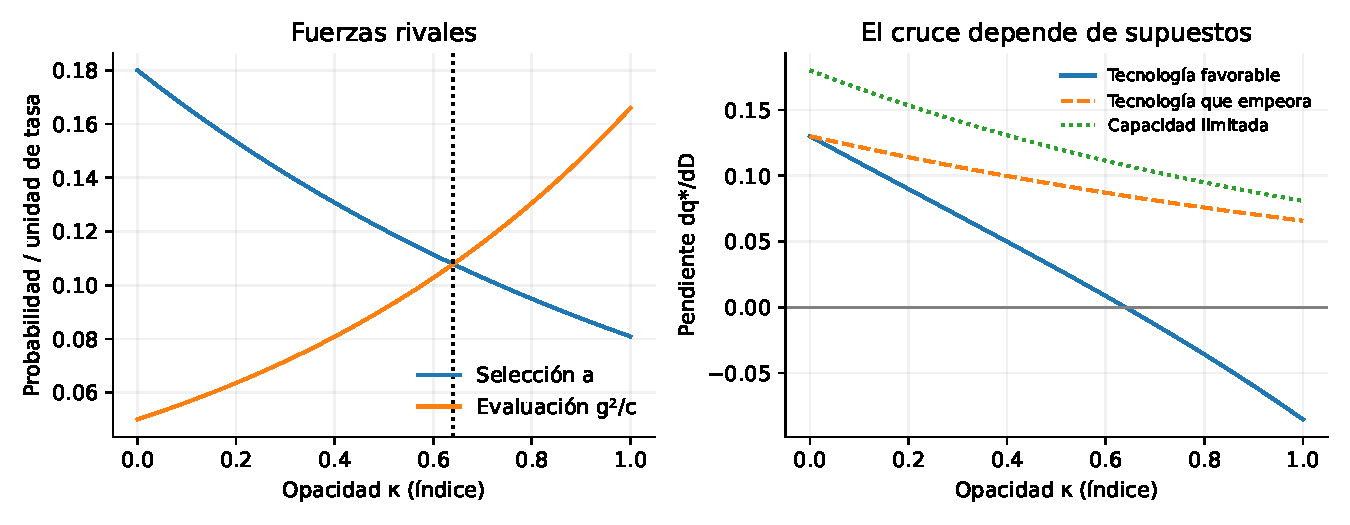
\includegraphics[width=\linewidth]{../code/figures/mechanisms.pdf}
\caption{Selección, evaluación y supuestos del cruce. La tecnología alternativa
usa $g=\sqrt{0.05}e^{-0.4\kappa}$; el costo sigue aumentando. Capacidad limitada:
$\bar e=0.08$. Fuente: simulación ilustrativa, \texttt{code/verify.py}.
Una unidad de pendiente se mide por unidad de tasa decimal.}\label{fig:mechanisms}
\end{figure}

La Figura~\ref{fig:mechanisms} incluye un escenario igualmente admisible en
el que $g$ cae: $H=0.05e^{-1.2\kappa}$. Entonces
$a/H=3.6e^{0.4\kappa}>1$ en todo el intervalo y no hay reversión. El código
también muestra que una capacidad de 0.08 mantiene pendiente positiva aunque
la tecnología de evaluación sea favorable. Son contraejemplos a una lectura
incondicional de que la opacidad invierte el signo.

\subsection{Esquinas y estabilidad}
La Figura~\ref{fig:corners} utiliza dos configuraciones adicionales.
Con $\bar q=0.35$, $a=0.04$, $g=0.4$, $c=1$ y $\bar e=0.44$, la restricción
de capacidad empieza a operar en $D=0$. A la izquierda, la pendiente de riesgo
es $0.04-0.16=-0.12$; a la derecha es $0.04$. La solución es continua, pero
no diferenciable en ese punto. En el segundo caso $\bar q=0.04$, $a=0.04$,
$g=0.5$, $c=1$ y $\bar e=1$ llevan al piso de riesgo, que detiene reducciones
adicionales. La igualdad de una FOC sin restricciones daría probabilidades
negativas en ese ejemplo y sería una solución inválida.

\begin{figure}[htbp]
\centering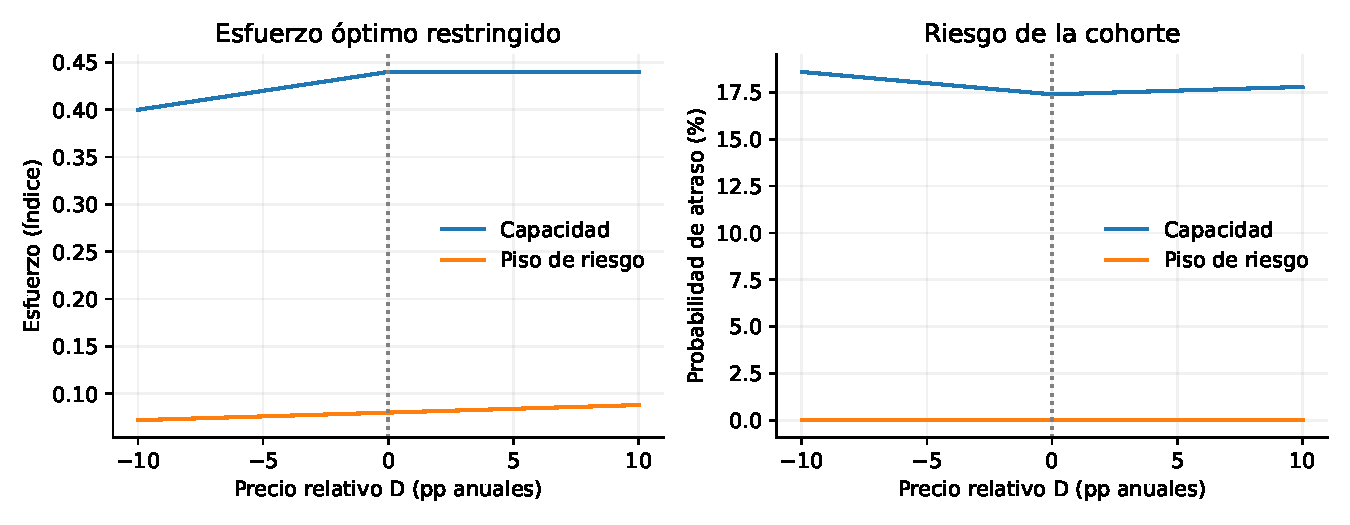
\includegraphics[width=.95\linewidth]{../code/figures/corners.pdf}
\caption{Esfuerzo y riesgo con capacidad y piso de probabilidad. $D$ en puntos
porcentuales anuales, riesgo en porcentaje. Fuente: \texttt{code/verify.py},
parámetros hipotéticos. El piso cero describe una frontera de la tecnología
lineal y no una recomendación de política.}\label{fig:corners}
\end{figure}

La solución analítica se compara con un optimizador acotado de SciPy que evalúa
directamente el objetivo e incluye ambos extremos como candidatos. De 1500
sorteos con semilla 20261110, 1495 son admisibles: 765 interiores, 293 de
capacidad y 437 de piso de riesgo. La máxima diferencia de esfuerzo fue
menor que $4\times10^{-8}$, con tolerancia exigida de $2\times10^{-6}$.
Las pendientes se contrastan con diferencias centrales de paso $10^{-6}$
solo cuando los tres puntos conservan régimen; el error máximo fue menor
que $1.1\times10^{-10}$. Se comprueba capacidad nula y se rechazan parámetros
con probabilidades inválidas, costo nulo, productividad negativa o pago no
positivo. Las comprobaciones necesarias lanzan excepciones ante una falla, por lo que
permanecen activas también al ejecutar Python con optimización.

\subsection{Contraejemplo de composición}
En $\kappa=0$, $D=0$, la evaluación interior da $q^*=0.225$ y
$\beta_D=\cohortSlope$. Tome $B_0=4$, $B_1=1$, $m_0=0.10$ y
$\varepsilon=3$. Así $w=0.2$ y
\[
M'=0.2[0.13-3(0.8)(0.225-0.10)]=\stockSlope<0.
\]
Todas las probabilidades y saldos son válidos. Una subida de un punto
porcentual tiene respuesta local de riesgo nuevo de 0.13 puntos porcentuales,
pero respuesta del ratio total de $-0.034$ puntos porcentuales. Son derivadas
locales, no efectos de un cambio discreto grande ni estimaciones causales.

\begin{figure}[htbp]
\centering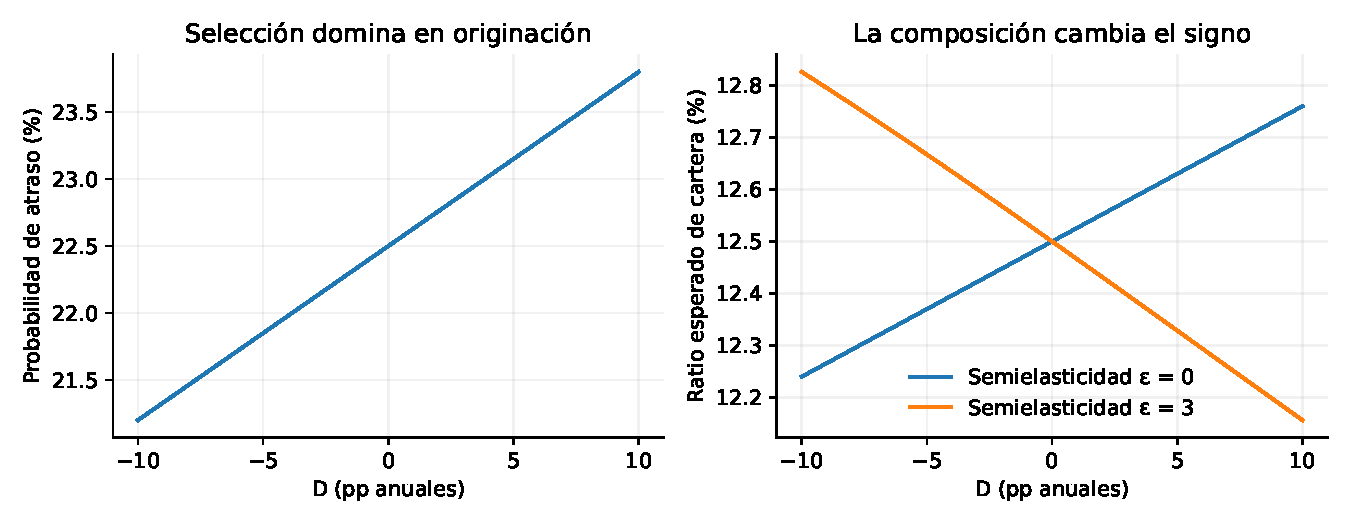
\includegraphics[width=\linewidth]{../code/figures/stock_composition.pdf}
\caption{Un mismo riesgo de cohorte puede asociarse con pendientes de saldo
opuestas. Con peso fijo ($\varepsilon=0$), el signo se transmite. Con volumen
sensible ($\varepsilon=3$), la composición domina. Fuente: simulación
ilustrativa, \texttt{code/verify.py}.}\label{fig:stock}
\end{figure}

La condición de P3 permite leer qué tan fuerte debe ser esa respuesta, sin
cambiar el modelo. En el punto del contraejemplo, $\beta_D=0.13$ y
$q^*-m_0=0.125$, por lo que, para cada peso positivo $0<w<1$,
\[
M'<0\quad\Longleftrightarrow\quad
\varepsilon>\frac{0.13}{(1-w)0.125}=\frac{1.04}{1-w}.
\]
Con $w=0.20$, el corte es $1.3$: por debajo predomina calidad, en el corte
ambos efectos se cancelan y por encima predomina composición. El valor
$\varepsilon=3$ se ubica en esta última región. La
Figura~\ref{fig:frontier} representa esa misma desigualdad para distintas
relaciones de saldos, manteniendo el riesgo y su pendiente en el punto
considerado. La región no es una frecuencia observada de bancos.

\begin{figure}[htbp]
\centering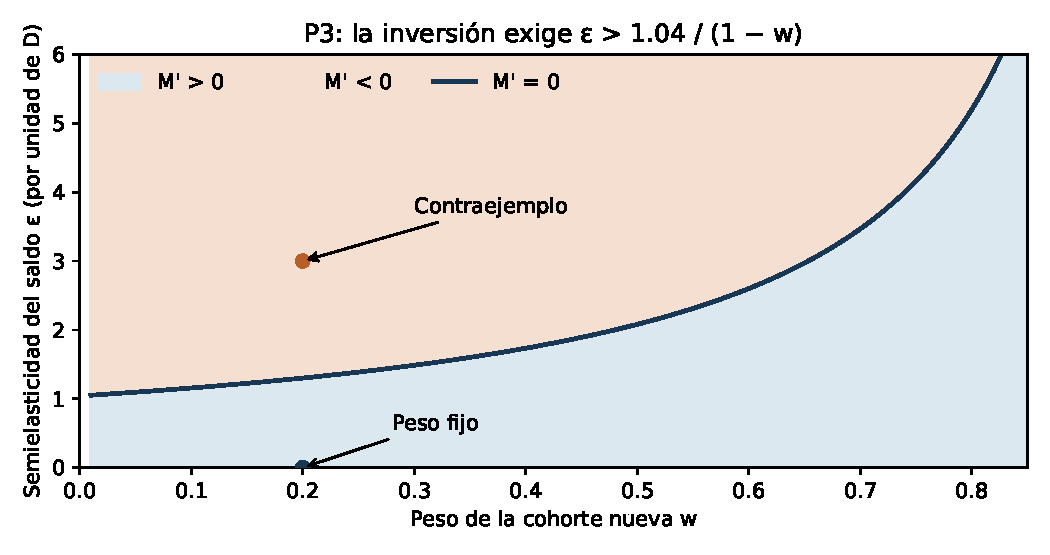
\includegraphics[width=.82\linewidth]{../code/figures/composition_frontier.pdf}
\caption{Frontera de inversión del signo de P3 en $D=0$, con
$\beta_D=0.13$ y $q^*-m_0=0.125$. Cada peso se obtiene con una relación
distinta de saldos positivos, fijos al tomar su derivada. La línea da
$M'=0$; encima $M'<0$ y debajo $M'>0$, para $0<w<1$. Fuente:
\texttt{code/reader\_checks.py}, llamado por \texttt{code/verify.py}.
Es el mismo ejercicio ilustrativo de la presentación, no un resultado nuevo.}\label{fig:frontier}
\end{figure}

La Proposición~\ref{p:stock} se contrasta en 51 valores de opacidad, 25 precios
y cuatro valores de $\varepsilon$, siempre con derivadas bien definidas. El máximo error
frente a diferencias finitas fue inferior a $3\times10^{-11}$. SymPy comprueba
por separado la regla del producto y la derivada del peso exponencial. Esta
doble comprobación reduce el riesgo de repetir un mismo error en una fórmula
y su implementación, aunque no reemplaza una prueba formal.

La verificación contiene 4018 comprobaciones base y 73 controles adicionales
de probabilidades de referencia, primitivas admisibles, saldos en nivel y
derivada, aritmética racional y signos a ambos lados de la frontera en
diecisiete pesos. Los resultados adicionales se registran en
\path{code/output/reader_verification.json}. Estos controles permiten detectar
errores de implementación en los casos examinados; la validez general de los
resultados descansa en las demostraciones.

\begin{figure}[htbp]
\centering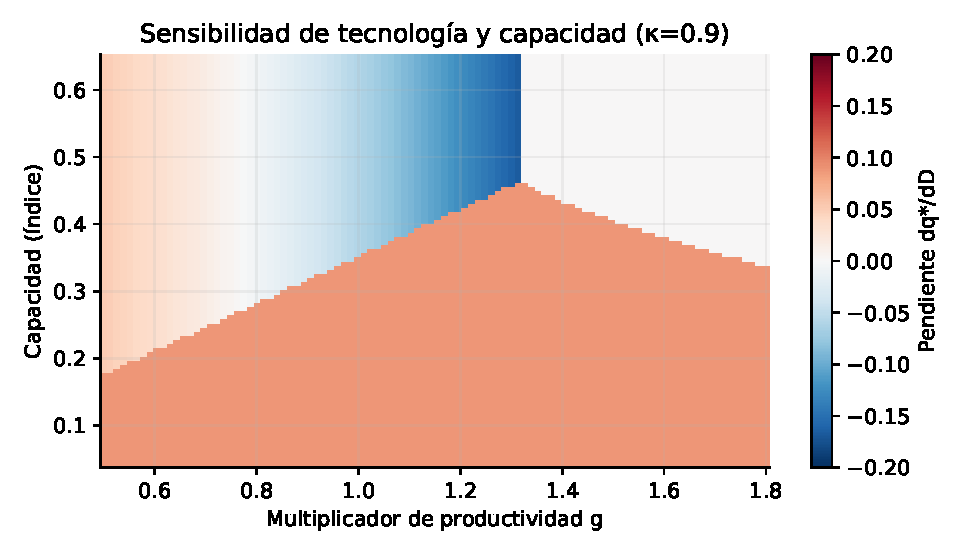
\includegraphics[width=.80\linewidth]{../code/figures/sensitivity.pdf}
\caption{Sensibilidad de la pendiente a productividad y capacidad con
$\kappa=0.9$. El mapa incluye los regímenes efectivos, incluido el piso de
riesgo; no extrapola una FOC interior fuera de su dominio. Fuente:
\texttt{code/verify.py}, simulación hipotética.}\label{fig:sensitivity}
\end{figure}

El mapa de la Figura~\ref{fig:sensitivity} varía capacidad y productividad,
manteniendo el resto de parámetros. Mejor productividad no implica una
pendiente negativa ilimitada: la saturación en riesgo cero la vuelve cero.
El ejercicio identifica regiones del modelo, no frecuencias con que ocurren
en bancos peruanos. Sin datos de evaluación no se puede asignar un banco a
una región a partir de su tasa observada.

\section{Discusión e implicaciones empíricas}
\subsection{Estática comparativa, predicción y causalidad}
La derivada $\partial_Dq^*$ compara problemas de evaluación con precios
cercanos: mantiene fijas las primitivas y permite reoptimizar el esfuerzo.
Es, por tanto, una estática comparativa condicional. Un coeficiente predictivo
de $M_{t+h}$ sobre $D_t$ resume, en cambio, una distribución conjunta de
precios, tecnología, composición y shocks. Un efecto causal de modificar el
precio exige además identificar una intervención y modelar las respuestas
de demanda y de los demás bancos. Son objetos distintos, aunque utilicen
las mismas variables observables.

La decisión de precios queda fuera del problema de continuación. En
consecuencia, el modelo caracteriza cómo responde la evaluación a un precio
dado, pero no determina qué precio se observa en equilibrio. Esta delimitación
permite aislar el mecanismo sin atribuir al resultado una interpretación
causal, una recomendación de fijación de tasas o una regla óptima de supervisión.

\subsection{Requisitos para evaluar el contenido predictivo}
Una evaluación empírica compatible con el modelo requiere un panel banco-mes,
tasas comparables por celda, pesos de saldo rezagados y cobertura documentada.
Un horizonte de doce meses permite estudiar el desempeño posterior, siempre
que el evento se mantenga definido de manera uniforme. La mora mayor de
noventa días, por ejemplo, debe tratarse como un objetivo distinto de la mora
contable cuando sus definiciones no coinciden.

La comparación relevante enfrenta un pronóstico basado en morosidad pasada
y ciclo económico con su ampliación mediante el precio relativo. Es necesario
separar el spread propio, definido como tasa del banco menos referencia, del
spread medio de pares, definido con la misma referencia. Como $D$ es la
diferencia entre ambos, incluir simultáneamente los tres regresores produce
colinealidad exacta. Esta identidad debe respetarse al especificar el contraste.

La cronología de información es igualmente decisiva. En un origen $t$, el
entrenamiento solo puede incorporar observaciones cuyo resultado a $t+h$ ya
se haya publicado. Por eso deben excluirse del extremo de la ventana los
horizontes aún desconocidos. Los pesos, escalas, tratamientos de faltantes y
reglas de comparabilidad deben estimarse con información pasada y fijarse
antes de evaluar. Si las series históricas están revisadas y no existen
versiones archivadas, el ejercicio corresponde a una evaluación en pseudo
tiempo real.

Ambos pronósticos deben evaluarse sobre los mismos bancos y fechas. La
dependencia entre entidades y la superposición de errores a horizontes largos
exigen un tratamiento explícito de la inferencia. La prueba de Clark--West
es una opción para modelos anidados bajo sus condiciones. Una reducción de
error constituye un resultado empírico que debe medirse; no se desprende de
las proposiciones. Del mismo modo, la ausencia de una mejora detectable puede
reflejar error de medición, poca potencia o cambios de régimen, además de la
información efectiva del precio.

\subsection{Supuestos que delimitan la interpretación}
La selección reducida y la tecnología lineal hacen transparente el mecanismo,
pero restringen su alcance. El esfuerzo no modifica el volumen de créditos y
los solicitantes y pares no eligen estratégicamente dentro del modelo. El
índice de opacidad tampoco proporciona, por sí mismo, una clasificación empírica
de segmentos. El cruce de P2 exige S4: sin esas condiciones, la opacidad puede
variar sin invertir la pendiente.

El puente de P3 exige además que evento, horizonte y saldo sean compatibles.
Castigos, curaciones, ventas de cartera, garantías o exposición cambiaria
pueden alterar la relación entre el riesgo nuevo y el ratio total. Los saldos
deterministas excluyen las covarianzas que aparecerían con un denominador
aleatorio. Restar tasas de pares o incorporar efectos fijos no sustituye esos
supuestos contables.

Estas restricciones orientan la aplicación del modelo. Para distinguir calidad
de composición es necesario observar cosechas y pesos; para atribuir una
respuesta a la evaluación se necesita información sobre esfuerzo o su
tecnología. Incorporar recuperaciones, evaluación cóncava o información
imperfecta del banco ampliaría el problema, pero requeriría volver a derivar
el óptimo y las condiciones de transmisión.

\section{Conclusiones}
El contenido informativo del precio relativo depende del mecanismo que
predomina y de la variable de riesgo que se observa. La solución global de la
decisión de evaluación muestra que la diferencia entre selección y evaluación
determina la pendiente únicamente en el interior. La capacidad y el piso de
probabilidad cambian esa regla, aun cuando la productividad de evaluar sea alta.
El umbral por opacidad requiere continuidad, descenso estricto, cruce e
interioridad; no es una consecuencia automática de la opacidad.

Al pasar de una cohorte al saldo total aparece un segundo margen: la
composición de cartera. La derivada del ratio agrega al efecto de calidad un
efecto de cambio de peso, que puede dominarlo e invertir su signo. Por ello,
una reducción de la morosidad agregada no implica necesariamente que haya
mejorado el riesgo de los créditos nuevos.

Para la supervisión de la banca peruana, el resultado precisa cómo interpretar
y contrastar una brecha de tasas: junto con la capacidad de evaluación, las
cosechas y la renovación del saldo. Las demostraciones y los ejercicios
reproducibles establecen las condiciones del mecanismo. Determinar cuánto
mejora el pronóstico requiere una evaluación empírica que respete las
definiciones y la información disponible en cada fecha.\label{body:end}
\clearpage
\bibliographystyle{plainnat}\bibliography{references}
\clearpage\appendix

\section{Reproducibilidad y material complementario}
Las demostraciones de las tres proposiciones se presentan completas en el
cuerpo del artículo. La guía \path{hand/guia_derivaciones.tex} organiza sus
manipulaciones algebraicas, reglas, condiciones y unidades. Es material
tipográfico de apoyo; no constituye evidencia de una revisión manuscrita
personal. Esa evidencia se distingue expresamente en \path{hand/README.md}.

El punto único de reproducción computacional, desde la raíz del repositorio, es:
\begin{verbatim}
python -m pip install -r code/requirements.txt
python code/verify.py
\end{verbatim}
Se regeneran las seis figuras en español e inglés, los archivos
\path{verification.json} y \path{reader_verification.json}, y las macros
numéricas utilizadas en el artículo. Las dependencias y la semilla están
fijadas. Las simulaciones no requieren credenciales ni conexión de red;
\path{code/data/README.md} documenta la fuente, las unidades y el universo
de la transcripción del BCRP. Los materiales de la presentación del tema se
conservan identificados como documentos históricos.

\section{Formalización de las proposiciones en Lean}\label{app:lean}
Las tres proposiciones tienen especificaciones transparentes y pruebas
generales en Lean 4.30.0-rc2. La formalización utiliza AppliedModelingLib y
la configuración \path{gpt-5.6-sol}, esfuerzo \path{xhigh}, exigida por el
curso. Los controles se ejecutan en Linux con el motor oficial sin parches.

\begin{center}\small
\begin{tabular}{L{.06\linewidth}L{.21\linewidth}L{.15\linewidth}L{.47\linewidth}}
\toprule P. & Declaración & Estado & Hipótesis y cobertura\\\midrule
P1 & \path{proposition1} & Probado & S1--S3: máximo único, fórmulas, cotas, regímenes, capacidad cero, continuidad y derivadas laterales.\\
P2 & \path{proposition2} & Probado & S1--S4: umbral interior único y signos de la derivada.\\
P3 & \path{proposition3} & Probado & S1--S3 y S5: identidad, derivada, conservación e inversión de signo.\\
\bottomrule\end{tabular}
\end{center}
Las declaraciones pertenecen al espacio \path{Galarza26RelativeCredit} y se
encuentran en \path{lean/ProofInterface.lean}. Cada una prueba el tipo exacto
definido en \path{lean/PaperInterface.lean}, con sufijo \texttt{Spec}. No se
introducen hipótesis matemáticas adicionales ni se utiliza \texttt{sorry}.
La clausura de axiomas de los tres endpoints contiene únicamente
\texttt{propext}, \texttt{Classical.choice} y \texttt{Quot.sound}.

La identificación exacta del PDF auditado, su commit, el resultado del
chequeo oficial y el grafo de evidencia se conservan en
\href{https://github.com/fgalarzac/ai-project/blob/main/docs/lean_progreso.md}{\path{docs/lean_progreso.md}}.
Este registro distingue la compilación de las pruebas, la correspondencia
con el texto y el cierre del protocolo. Su ubicación externa permite fijar
la fuente sin una referencia circular a su propia huella digital. Las
ediciones española e inglesa expresan el mismo modelo y los mismos resultados;
el registro identifica expresamente la fuente sometida a validación.

La verificación formal establece consecuencias de las definiciones y los
supuestos. No acredita que los bancos peruanos satisfagan S5, ni identifica
efectos causales o mejoras predictivas. Tampoco sustituye la comprobación
personal de las derivaciones.

\clearpage
\section{Colaboración con inteligencia artificial}
El registro \path{prompts.md} conserva las interacciones literales disponibles
y distingue los resúmenes de los textos originales. La tabla siguiente
documenta afirmaciones relevantes, el veredicto aplicado y la comprobación
que lo sustenta. Estos controles computacionales no se atribuyen a una
revisión manuscrita del autor que carezca de evidencia documental.

\begin{longtable}{L{.29\linewidth}L{.29\linewidth}L{.33\linewidth}}
\toprule Afirmación o aporte & Veredicto y fundamento & Comprobación\\\midrule
\endhead
El problema de dos etapas está resuelto. &
Incompleto: el precio es un dato; la optimización corresponde al esfuerzo. &
Definición del problema de continuación y prueba global de P1.\\
La pendiente $a-g^2/c$ rige para todo precio. &
Falso fuera del interior: la capacidad produce pendiente $a$ y el piso, cero. &
P1, optimizador independiente y ejemplo de capacidad.\\
La opacidad mejora necesariamente la evaluación. &
No es una implicación general: $2g'/g-c'/c$ puede ser negativo. &
Identidad \eqref{eq:logs} y escenario sin cruce.\\
El signo del riesgo nuevo pasa al ratio de saldo. &
Condicional: los pesos y el riesgo antiguo deben satisfacer las restricciones de P3. &
Identidad de composición y contraejemplo con $M'=-0.034$ y $q^{*\prime}=0.13$.\\
Restar pares elimina toda exposición común. &
Excesivo: se cancela la base aditiva, pero pueden persistir cargas heterogéneas. &
Descomposición con coeficientes $\lambda_j$.\\
Las cifras del plan equivalen a estimaciones reproducidas. &
Se excluyen del análisis empírico al no existir una base consolidada reproducible en los materiales. &
Separación entre estadísticas públicas documentadas y parámetros ilustrativos.\\
Las simulaciones demuestran los resultados generales. &
Falso: comprueban implementaciones y pueden detectar errores en los casos examinados. &
Demostraciones completas, controles independientes y pruebas Lean.\\
Un punto porcentual de precio cambia el riesgo previo en $0.01a$ unidades. &
Correcto: equivale a $a$ puntos porcentuales de riesgo. &
Conversión de unidades en S1 y ejemplo con $a=0.18$.\\
\bottomrule
\end{longtable}

\section{Disponibilidad de materiales}
Las fuentes LaTeX, ambas ediciones del artículo, las figuras, el código y los
artefactos de formalización se distribuyen en el repositorio público citado
en la primera página. \path{docs/fuentes.md} detalla la procedencia y el
alcance de la verificación de cada fuente. Los documentos de propuesta y
presentación conservan sus fechas y definiciones originales; el artículo
identifica la especificación empleada en los resultados finales.
\end{document}
